\section{Visualization}
\label{sec:viz}

\begin{figure*}[t]
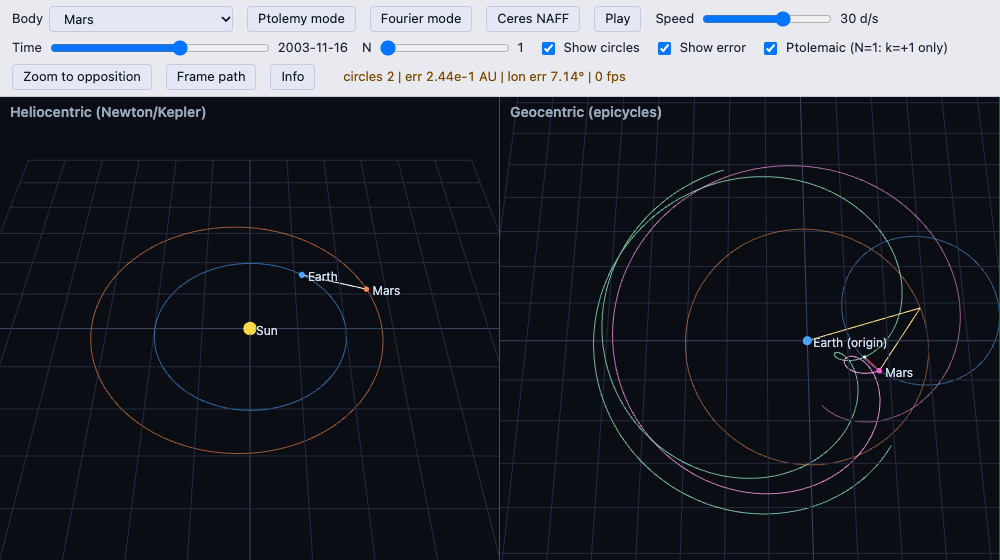
\includegraphics[width=\textwidth]{fig_spa_screenshot.png}
\caption{Screenshot of the interactive viewer (URL parameters
\texttt{preset=ptolemy\&t=2452960\&N=1\&info=0}: Mars, Julian date 2452960,
Ptolemaic $k=+1$ subset only, error shown). Left: heliocentric Newtonian view.
Right: geocentric view with the epicycle chain (yellow arm), its two circles,
the trail of the chain tip, the exact geocentric path (green) and the error
vector (red) between the chain tip and true Mars. The readout (top) shows the
circle count and the error against exact Kepler motion (here $0.244$~AU,
$7.14^\circ$ in longitude).}
\label{fig:spa}
\end{figure*}

To make the construction tangible we provide an open-source interactive
viewer, a single-page web application (TypeScript and three.js) in the
\texttt{web/} directory of the repository. Figure~\ref{fig:spa} shows it. Two
three-dimensional views are synchronized to one clock. The left view is
heliocentric and Newtonian: the Sun, the Earth and the chosen body move on
their Kepler ellipses. The right view is geocentric, centred on the Earth,
and shows the epicycle chain: the deferent, the successive epicycles drawn
as circles in their own orbital planes, the arm joining their centres, and
the trail of the chain tip. In the left panel a line joins the Earth to the body; it is
the geocentric vector whose epicycle sum is drawn in the right panel.

The geocentric chain is computed live in the browser, by a TypeScript port
of the Kepler and Bessel-coefficient code of Sec.~\ref{sec:num-expansion}
that is tested against golden values generated by the Python reference.
Nothing is precomputed or fitted: the radii, planes and angular rates are the
analytic quantities of Sec.~\ref{sec:theory}, determined by the orbital
elements. The slider $N$ ($1$ to $60$) sets the truncation order for both the
body and the Earth, so the viewer demonstrates the convergence of
Sec.~\ref{sec:res-conv} directly: at $N=1$ one sees the Ptolemaic
deferent-and-epicycle picture with its visible displacement, and as $N$
increases the chain tip converges onto the heliocentric truth and the small
circles shrink. A live readout shows the number of circles and the
instantaneous error against exact Kepler motion, in AU and as a
longitude error. The state is encoded in URL parameters (\texttt{t}, a Julian
date, \texttt{N}, \texttt{speed} in days per second, and \texttt{paused}) so that a configuration can be shared.
Intended uses are as a classroom demonstration of what ``epicycles are
Fourier series'' means quantitatively, and of how fast the series converges
for planet-like eccentricities.

